% Capítulo 1 - Introducción a los Sistemas de Bases de Datos

\section{Motivación}
Primero que nada, sería bueno contestar la mítica pregunta que harían algunas personas: \textit{¿Y por qué no simplemente almacenas todo en un Excel / documento de texto / papel?} A veces puede no ser inmediatamente obvio el propósito de un sistema de bases de datos.

\begin{figure}[h]
  \centering
  \includegraphics[width=0.3\textwidth]{img/foldermess.png}
  \caption{Almacenamiento de datos análogo}
\end{figure}

Muchas veces los métodos pueden ser demasiado desorganizados, lentos para realizar búsqueda, ineficientes con el uso del espacio y en los peores casos, poco confiables. Por esto, resulta importante usar bases de datos, que se deben enfocar en resolver estos problemas.

Sin embargo, considerando todo esto, aún faltan cosas para implementar un \textit{buen} sistema de bases de datos. Perfectamente un sistema de bases de datos que resuelve todas las cosas que hemos descrito anteriormente, que por ejemplo, se puede basar en almacenar los datos en un \texttt{.txt} va a presentar los siguientes problemas
\begin{itemize}
  \item Organización ineficiente de los datos.
  \item Búsqueda costosa de los datos por falta de uso de índices.
  \item Fuerza bruta para procesar las consultas.
  \item No hay manejo de buffer: Todo se va a la RAM, colapsando el sistema muy rápido.
  \item Falta de control de concurrencia: Si más de un actor usa la base de datos simultáneamente, \textbf{caos}.
  \item No es capaz de recuperarse de una falla: Se perderán datos si, por ejemplo, se corta la luz.
  \item Falta de seguridad.
  \item No paralelizable.
\end{itemize}

Algunos buenos motivos para tratar de comprender muy bien el funcionamiento de los sistemas de bases de datos (que nos permitirá crear un buen sistema de bases de datos) son los siguientes:
\begin{itemize}
  \item Big Data y Data Deluge: Hoy en día estamos produciendo datos muy rápido\dots Al punto en que estamos teniendo problemas para poder procesarlos e interpretarlos de manera correcta. No sirve de nada tener un montón de datos si no podemos hacer nada con ellos.
  \item Manejar datos es muy importante: ¿No me crees? Pregúntale a las plataformas grandes de internet, como redes sociales masivas como X (twitter jeje), Instagram, Facebook, etc. Manejar volúmenes gigantes de datos es algo muy importante para ellos (si no, sus plataformas simplemente no funcionarían). Practicamente cualquier negocio hoy en día se basa en datos. Si hace mucho tiempo atrás existió la fiebre del oro, hoy en día estaríamos en algo así como la fiebre de los datos.
  \item La herramienta más usada para trabajar con datos: Saber trabajar con sistemas de bases de datos es un skill que se usa mucho hoy en día en el mundo laboral. Es extremadamente solicitado.
\end{itemize}

\makeobservationbox{Mi abuelo siempre me decía\dots}{
  “Las técnicas para el manejo y gestión eficiente de datos representan
  hoy en día una herramienta fundamental que puede ayudarles a
  ustedes, los futuros ingenieros o científicos de datos, para utilizar
  el poder inherente en los datos y transformarlos en conocimiento.”
}

\section{El Modelo Relacional}
\subsection{Anatomía de una Relación}
Una relación $R$ se compone de
\begin{itemize}
  \item Esquema: \texttt{name(att$_1$: $D_1$, \ldots, att$_n$: $D_n$)}, donde
  \begin{itemize}
    \item \texttt{name}: Nombre de la relación. Por ejemplo, el nombre de la \texttt{TABLE} en PostgreSQL.
    \item \texttt{att$_i$}: Nombre del atributo $i$.
    \item $D_i$: Dominio del atributo $i$. Que datos son los que almacenamos en ese atributo (números, strings, fechas, vectores, etc).
    \item $n$: Cantidad de atributos de la relación $R$.
  \end{itemize}
  \item Instancia: Subconjunto finito de $D_1 \times \ldots \times D_n$. Esto es al final la tupla en cuestión con los datos.
\end{itemize}

\makeobservationbox{Observación}{
  Dada una relación $R$, usaremos las siguientes expresiones para referirnos a ciertos aspectos.
  \begin{itemize}
    \item $R$: El nombre y la instancia de la relación $R$.
    \item schema($R$): El esquema de la relación $R$.
    \item arity($R$): La cantidad de atributos de la relación $R$.
    \item dom(\texttt{att}$_i$): El dominio $D_i$ del atributo \texttt{att}$_i$.
  \end{itemize}
}

Una relación $R$ se puede representar por medio de una tabla.

\begin{figure}[h]
  \centering
  \begin{tabular}{|c|c|c|c|}
    \hline
    \texttt{att$_1$} & \texttt{att$_2$} & \ldots & \texttt{att$_n$} \\\hline
    $v_1$ & $v_2$ & \ldots & $v_n$ \\\hline
    $v'_1$ & $v'_2$ & \ldots & $v'_n$ \\\hline
    \ldots & \ldots & \ldots & \ldots \\\hline
  \end{tabular}
  \caption{Tabla representante de una relación $R$.}
\end{figure}

En este ejemplo, $\vec{v};\ \vec{v'}$ corresponden a tuplas de $R$. Cabe destacar que aquí el orden de las filas no es importante y cada tupla es diferente al resto. Claramente se pueden repetir datos entre las tuplas, pero siempre tiene que haber por lo menos un atributo que sea diferente.

\subsection{Base de Datos Relacional}
Una base de datos relacional $\mathcal{D}$ consiste en un conjunto de relaciones, cada una con un nombre distinto.
\[ \mathcal{D} = \{R_1, R_2, \ldots, R_m\} \]

Un esquema relacional $\mathcal{S}$ de una base de datos relacional $\mathcal{D}$ consiste en el conjunto de esquemas de todas las relaciones que componen a $\mathcal{D}$.
\[ \mathcal{S} = \text{schema}(\mathcal{D}) = \{ \text{schema}(R_1), \text{schema}(R_2), \ldots, \text{schema}(R_m) \} \]

\makeobservationbox{Otras definiciones}{
  \begin{itemize}
    \item $dom(\mathcal{S})$: Todas las bases de datos que tienen como esquema relacional a $\mathcal{S}$.
    \item $|R|$: Número de tuplas en $R$ (cardinalidad).
  \end{itemize}
}

\subsection{Restricciones de Integridad y Validez de una Base de Datos}
Una restricción de integridad consiste en una condición $\varphi$ que restringe los datos que pueden ser almacenados en una base de datos relacional.

De esto, podemos derivar el concepto de validez de una base de datos. Se dice que una base de datos es válida respecto a $\varphi$ si es que satisface la restricción impuesta por $\varphi$.
\[ \mathcal{D} = \varphi \]

\subsection{Extracción de datos a base de consultas}
Primero que nada, debemos dejar en claro \textit{qué es} una consulta. Para nosotros, una consulta consiste en una función de tipo
\[ f:\ dom(\mathcal{S}) \rightarrow D \]
donde $S$ es un esquema relacional y $D$ es un dominio cualquiera.

De aquí podemos extrapolar el concepto de lenguaje de consultas. Esto es un conjunto de expresiones sintácticas que definen una consulta por medio de una semántica. Aquí nos enfocaremos en SQL y Algebra Relacional.

\section{SQL (Structured Query Language)}
Es actualmente el estándar mundial para consultas a bases de datos relacionales. Esto se usa en todos lados (como mi ejemplo favorito, PostgreSQL). Este es un lenguaje de consultas declarativo, basado en cálculo relacional. Este lenguaje tiene varios componentes.
\begin{itemize}
  \item Data Definition Language (DDL): \texttt{CREATE}, \texttt{ALTER}, etc.
  \item Data Manipulation Language (DML): \texttt{SELECT}, \texttt{INSERT}, \texttt{DELETE}, etc.
  \item Data Control Language (DCL): \texttt{GRANT}, \texttt{REVOKE}, etc.
\end{itemize}

Una consulta SQL sigue una estructura general que se ve más o menos así:
\begin{minted}{sql}
SELECT <atributos>
FROM <relaciones>
WHERE <condiciones>;
\end{minted}

De aquí aparecen las consultas anidadas. Estas son consultas que contienen dentro de sí, una consulta embebida. Usualmente esto se da en expresiones como \texttt{WHERE}, \texttt{FROM} o \texttt{HAVING}
\begin{tcolorbox} [
  width=\textwidth,
  title={Ejemplo},
  colbacktitle=gray
]
  \begin{minted}{sql}
SELECT pName, pGoals
FROM Players
WHERE pGoals = (
  SELECT MAX(pGoals)
  FROM Players
);
  \end{minted}
  Resultado: El nombre y la cantidad de goles del jugador con más goles a su nombre.
\end{tcolorbox}

Existe un tipo particular de consulta anidada, llamada consulta correlacionada, la cual contiene una subconsulta por medio de una referencia a una consulta externa.
\begin{tcolorbox} [
  width=\textwidth,
  title={Ejemplo},
  colbacktitle=gray
]
  \begin{minted}{sql}
SELECT pName, pYear
FROM Players as P
WHERE 1 <= (
  SELECT AVG(mGoals)
  FROM Matches as M
  WHERE M.mId = P.pId
);
  \end{minted}
  Resultado: El nombre y el año de los jugadores que meten en promedio más de un gol en un partido.
\end{tcolorbox}

\section{Álgebra Relacional}
Este consiste en un lenguaje para realizar consultas en bases de datos relacionales basado en operadores relacionales.

\subsection{Operadores Relacionales}
\subsubsection{Selección $\sigma_\theta(R)$}
Operador que filtra las tuplas que se obtendrán de la consulta. Es un equivalente al \texttt{WHERE} en SQL.

Aquí, $\theta$ es una combinación booleana de términos:
\begin{center}
  atributo$_1$ op atributo$_2$\\
  atributo op constante
\end{center}
donde $\text{op} \in \{ =, \leq, \geq, <, > \}$.

\subsubsection{Proyección $\pi_L(R)$}
Operador que elige los atributos que se obtendrán al final de la consulta. Es un equivalente al \texttt{SELECT} en SQL.

En este operador, $L$ corresponde a una lista de atributos presentes en la relación $R$.

\subsubsection{Joins}
Este tipo de operador se encarga de mezclar dos relaciones.
\begin{itemize}
  \item Producto cruz: $R_1 \times R_2$
  \item $\theta$-join: $R_1 \bowtie_\theta R_2 = \sigma_\theta(R_1 \times R_2)$
  \item Equi-join: $R_1 \bowtie_\phi R_2 = \sigma_\phi(R_1 \times R_2)$, donde $\phi$ solo contiene igualdades.
  \item Natural-join: $R_1 \bowtie_\phi R_2 = \sigma_\phi(R_1 \times R_2)$, donde $\phi = \bigwedge_{a \in \texttt{att}(R_1) \cap \texttt{att}(R_2)} R_1.a = R_2.a$
\end{itemize}

\subsection{Álgebra Relacional Extendida}
Se agregan algunos operadores extra que no son parte del álgebra relacional tradicional con el fin de permitir hacer algunos procesos que son necesarios hoy en día.
\begin{itemize}
  \item Renombrar: $\rho_{\texttt{old\_att} \rightarrow  \texttt{new\_att}}(R)$
  \item Eliminar duplicados: $\delta(R)$
  \item Group-by con agregación: $\gamma_{G, A}(R)$, donde $G$ es la lista de atributos a agrupar, y $A$ es una lista de elementos de la forma $f(\texttt{agg\_att} \rightarrow \texttt{new\_att})$ con $f \in \{ \texttt{MIN}, \texttt{MAX}, \texttt{SUM}, \texttt{AVG}, \ldots \}$
  \item Sorting: $\tau(R)$
\end{itemize} 
\pagebreak

\subsection{Plan lógico}
El plan lógico consiste en un árbol de parsing, el cual da el primer paso para poder evaluar una consulta.
\begin{figure}[h]
  \centering
  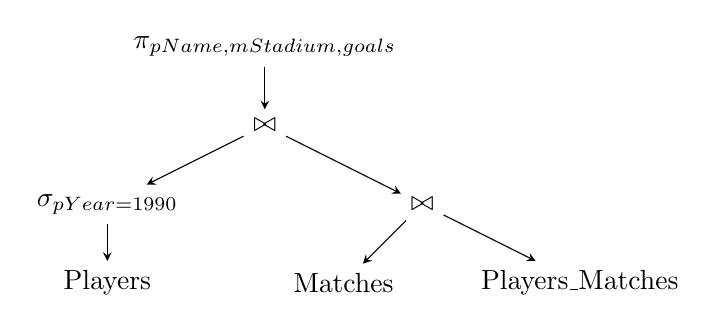
\begin{tikzpicture}
    \node (projection) at (0,0) {$\pi_{\text{pName, mStadium, goals}}$};
    \node (bowtie1) at (0,-1) {$\bowtie$};
    \node (select) at (-2,-2) {$\sigma_{\text{pYear = 1990}}$};
    \node (players) at (-2,-3) {Players};
    \node (bowtie2) at (2,-2) {$\bowtie$};
    \node (matches) at (1,-3) {Matches};
    \node (playersmatches) at (4,-3) {Players\_Matches};
    
    
    \draw[-stealth] (projection) -- (bowtie1);
    \draw[-stealth] (bowtie1) -- (select);
    \draw[-stealth] (select) -- (players);
    \draw[-stealth] (bowtie1) -- (bowtie2);
    \draw[-stealth] (bowtie2) -- (matches);
    \draw[-stealth] (bowtie2) -- (playersmatches);
  \end{tikzpicture}
  \caption{Ejemplo de un plan lógico}
\end{figure}

